\section{Wstęp}

\begin{frame}{Wstęp}
  \begin{block}{}
    $$ f(x) = \sum_{i=0}^m a_i \cdot x^i = 0; \qquad a_m \neq 0 $$
  \end{block}

  \begin{itemize}
    \item Wielomian stopnia $m$ -- $m$ pierwiastków,
    \item Jeżeli $a_i$ -- rzeczywiste, to ewentualne pierwiastki zespolone są parami sprzężone:
    $$ \alpha + \textit{\textrm{i}} \cdot \beta, \quad \alpha - \textit{\textrm{i}} \cdot \beta $$
    \item Jeżeli $a_i$ -- zespolone, to brak związku między pierwiastkami.
  \end{itemize}
\end{frame}

\begin{frame}
  Szukanie zer -- dobór metody:
  \begin{itemize}
    \item Dowolny
    \item Ze względu na postać $f(x)$ -- metody specjalne (zwłaszcza dla w. zespolonych).
  \end{itemize}

  Trudności:
  \begin{itemize}
    \item Wielokrotne pierwiastki -- trudno ,,obramować'', łatwiej, gdy znana krotność,
    \item Blisko położone pierwiastki -- trudności jak wyżej.
  \end{itemize}

  \textit{Nie wiadomo z góry, jaki typ patologii wykazuje wielomian.}

  \vspace{5px}

  \begin{alertblock}{Uwaga}
      \textit{Zadanie wyznaczania zer wielomianów może być źle uwarunkowane.} (Wilkinson).
  \end{alertblock}
  % Wilkinson: rozwinąć temat
\end{frame}

\begin{frame}
  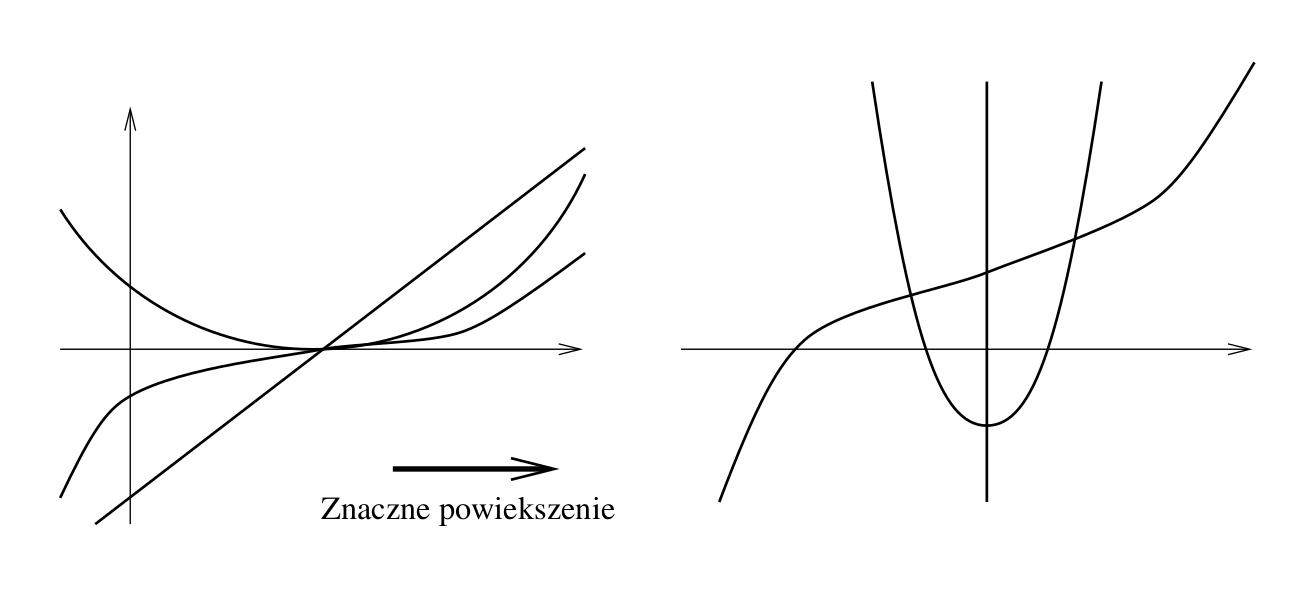
\includegraphics[width=\textwidth]{img/8/wielomian}
\end{frame}
